\documentclass[../main.tex]{subfiles}
\begin{document}
\section{Results}\label{results}
%oppgave 5b)
\subsection{Euler and Verlet without oo}
In order to make sure that our algorithm is running correctly, we will start solving the differential equation using both Euler's and Verlet's method without using object oriented(oo) code. The algorithms used to calculate the two are located in the following folders (\href{https://github.com/kmaasrud/Project-5/tree/master/code/Earth-Sun_Euler-FWD}{(Euler)} and \href{https://github.com/kmaasrud/Project-5/tree/master/code/Earth-Sun_Verlet}{(Verlet)})

\begin{figure}[!h]
  \centering
  \parbox{5cm}{
  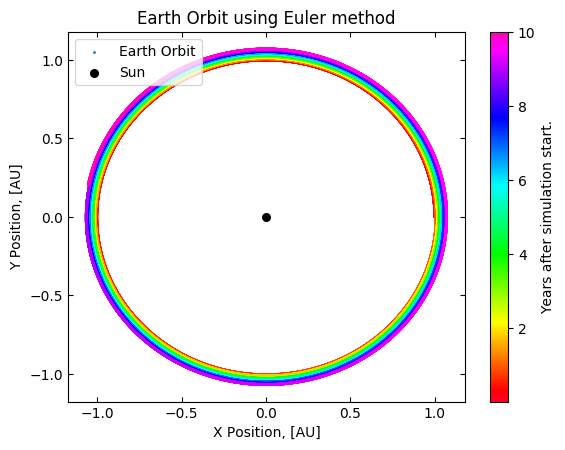
\includegraphics[width=5cm]{EarthOrbit_Euler.png}
  \caption{Earth orbit around the Sun using Eulers method}
  \label{fig:EarthOrbit_Euler}}
  \qquad
  \begin{minipage}{5cm}
    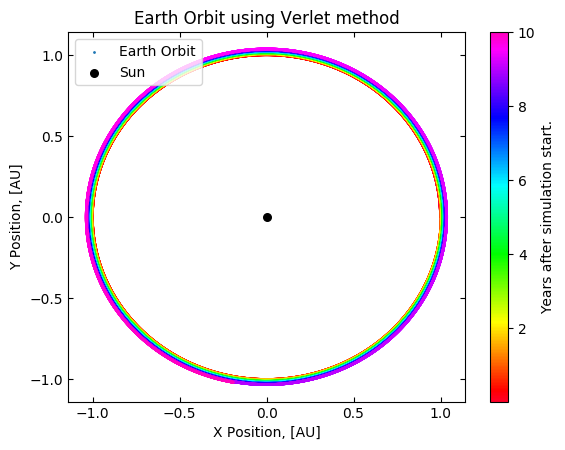
\includegraphics[width=5cm]{EarthOrbit_Verlet.png}
    \caption{Earth orbit around the Sun using Verlet's method}
    \label{fig:EarthOrbit_Verlet}
  \end{minipage}
  \end{figure}
\FloatBarrier

%skriv litt om programflow

%oppgave 5c)


\subsection{Testing}
\subsubsection{Stability with varying timestep} \label{sec:results-test-timestep}
In the figures below we plotted Earths orbit over a thousand years with different timesteps.

\begin{figure}[!h]
  \centering
  \makebox[\textwidth][c]{
  \begin{minipage}{0.7\textwidth}
        \centering
        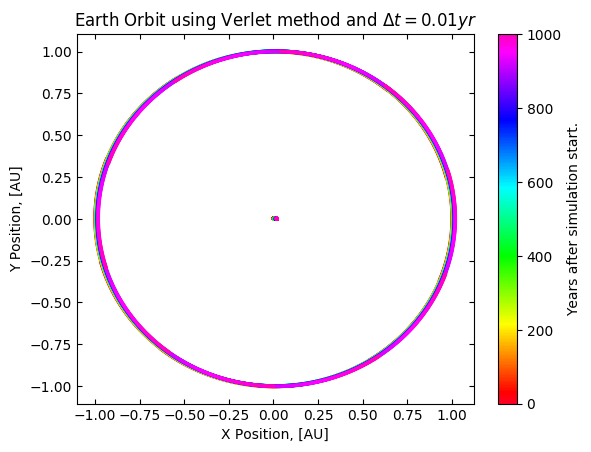
\includegraphics[width=1\textwidth]{/test/Earth-Sun_Test0-01.png} % first figure itself
    \end{minipage}\hfill
    \begin{minipage}{0.7\textwidth}
        \centering
        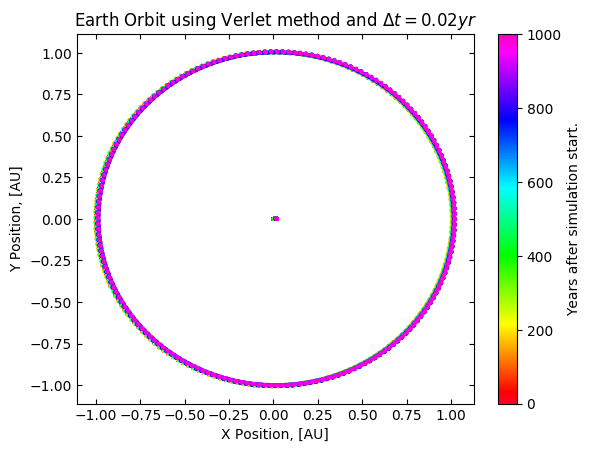
\includegraphics[width=1\textwidth]{/test/Earth-Sun_Test0-02.png} % second figure itself
    \end{minipage}
}
  \caption{Earth orbit with time steps $\Delta t = 0.01$years and $0.02$years respectively }
  \label{fig:results-Timestep1}
\end{figure}
\FloatBarrier
\begin{figure}[!h]
  \centering
  \makebox[\textwidth][c]{
  \begin{minipage}{0.7\textwidth}
        \centering
        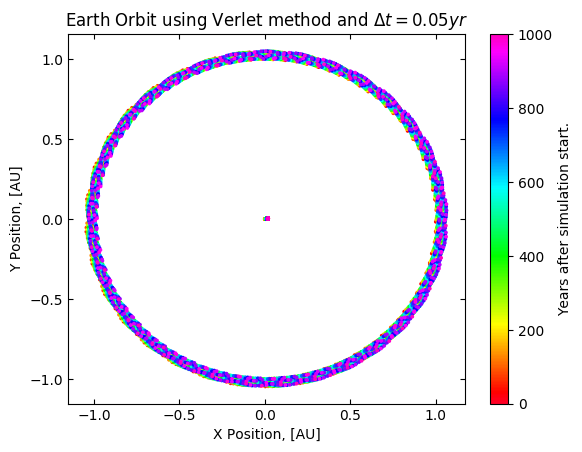
\includegraphics[width=1\textwidth]{/test/Earth-Sun_Test0-05.png} % first figure itself
    \end{minipage}\hfill
    \begin{minipage}{0.7\textwidth}
        \centering
        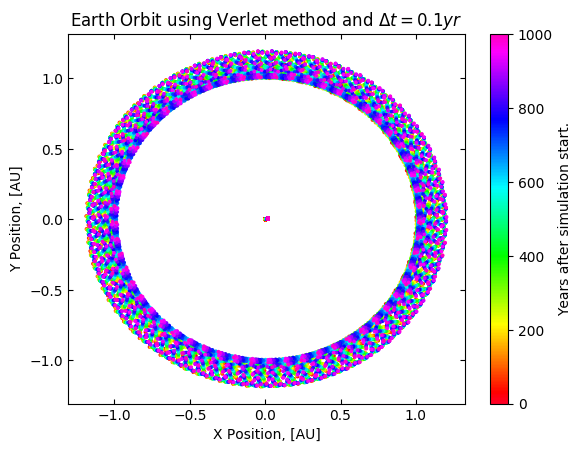
\includegraphics[width=1\textwidth]{/test/Earth-Sun_Test0-1.png} % second figure itself
    \end{minipage}
}
  \caption{Earth orbit with time steps $\Delta t = 0.05$year and $0.1$year respectively }
  \label{fig:results-Timestep2}
\end{figure}
\FloatBarrier

\subsubsection{Energy and angular momentum conservation}\label{sec:results-test-conservation}
In the figures below, kinetic energy and potential energy is plotted as a function of time in the system. We chose to simulate over a thousand years with a timestep of $\Delta t = 0.01$, as this gives the most stable results.
\begin{figure}[!h]
  \centering
  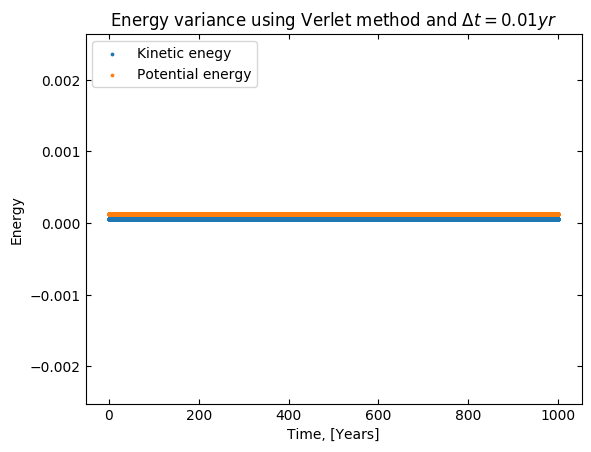
\includegraphics[width=1\textwidth]{/test/Energy_Test.png} % first figure itself
  \caption{Kinetic and Potential energy with timestep $\Delta t = 0.01$year.}
  \label{fig:results-Energies}
\end{figure}
\FloatBarrier

\subsubsection{Verlet vs. Euler}\label{sec:Verlet_VS_Euler}
\begin{table}[!h]
  \caption{Comparison of flops and time for the Verlet and Euler method for 100000 iterations over a period of 10 years}
  \centering
  \begin{tabular}{l r r}
                            &\textbf{Flops}&\textbf{Timing}\\
    Euler's method:          &10N&2580 ms\\
    Verlet's method:          &6N&2875 ms\\
  \end{tabular}
  \label{tab:EulervsVerlet}
  \end{table}
\FloatBarrier

%oppgave 5 d)
\subsection{Escape velocity}
By trail and error the escape velocity of planet Earth is:
From section \ref{sec:theory} using equation \ref{eq:escapevelocity} to calculate the  theoretical value $$v_{esc-theoretical} = \sqrt{\frac{2\cdot4\pi^2\cdot1}{1}} = 2.83 \pi$$\

\begin{figure}[h!]
  \centering
  \includegraphics[width=6cm]{Earth-Sun_escape.png}
  \caption{Escape velocity of planet Earth}
  \label{fig:v_esc}
\end{figure}

We also looked at what happens when changing the exponent of the denominator the force of gravity from 2 towards 3 with initial velocity $v_{initial,x} = 2.2\pi$. This is shown in the following plots.

\begin{figure}[h!]
  \centering
  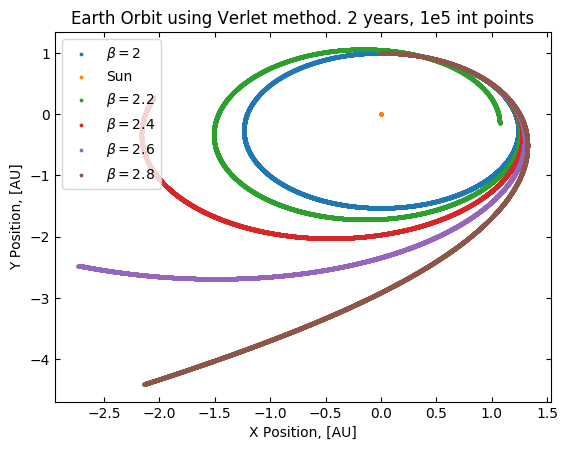
\includegraphics[width=6cm]{Earth-Sun_beta.png}
  \caption{Escape velocity with increasing exponent of denominator}
  \label{fig:v_esc_beta}
\end{figure}

%oppgave 5e)
\subsection{Three-body problem- Sun, Earth and Jupiter.}

% \begin{figure}
%   \includegraphics{}
%   \caption{Positions of Earth and Jupiter using the velocity Verlet method}
%   \label{fig:SunEarthJupiter}
% \end{figure}
%
% Stability Verlet solver
%
% \begin{figure}[!h]
%   \centering
%   \makebox[\textwidth][c]{
%   \begin{minipage}{0.7\textwidth}
%         \centering
%         \includegraphics[width=1\textwidth]{} % first figure itself
%     \end{minipage}\hfill
%     \begin{minipage}{0.7\textwidth}
%         \centering
%         \includegraphics[width=1\textwidth]{} % second figure itself
%     \end{minipage}
% }
%   \caption{Positions of Earth and Jupiter using the velocity Verlet method with an increase of mass of a factor 10 and 100 respectively}
%   \label{fig:jupiterincreasedM}
% \end{figure}

Stability Verlet solver with increased mass:

%oppgave 5f)
Sammenlign resultetene med de tidligere.


\end{document}
